\section{Planteamiento de la solución}
\subsection{Lenguaje para el manejo del mapa}
Como se quiere crear un mapa de la casa, donde se muestra los cada entidad de la casa, entonces se procederá a crear un lenguaje con una base de datos geográfica, tipo orientada a objetos, gracias a este se puede crear los suscriptores de forma dinámica, y poder crear modelos genéricos , para crear un comportamiento estándar para cualquier casa, poder cambiar estados y mostrar los estados de la casa, ademas de poder crear la estructura de la casa a través de un dibujo.\\
Esto contara con:
\subsubsection{Definidor de datos}
Este sera el encargado de que el software cree el mapa, creara la estructura de la casa, tomando en cuenta las entidades, el tipo entidad, las entidades con las que están unidas, cada entidad estará reverenciada por un código y una posición en el mapa para la hora del render del mapa.
\subsubsection{Manipulador de datos}
Gracias a este se actualizara y eliminaran los datos de las entidades cuando sea necesario, y a su vez todos los cambios serán utilizados por el manejador de IOT, para así poder hacer el buen control de las tareas de cada entidad de la casa.
\subsubsection{Consultor de datos}
Es el encargado de consultar las entidades de la casa por su id y tipo, este mostrara los datos de la entidad  y los datos de las entidades relacionadas con esta.

\subsection{Interfacez de usuario}
\subsection{Web Services}
lorem ipusm jdieuq jdakjskad jjkasdkaskjkjakd jdkasjkdas
\subsection{Capa de seguridad}
lorem ipusm jdieuq jdakjskad jjkasdkaskjkjakd jdkasjkdas
\subsection{Manejador IOT}
Esta funcionara gracias al lenguaje para el manejo del mapa, gracias a este se creara las suscripciones de la casa por tipo usando el protocolo MQTT con Eclipse Mosquitto, y gracias a este poder hacer la comunicación machine to machine, "maquina a maquina" para poder intelectual con las entidades desde los servicios web.
\subsection{Casos De Uso}
Primer caso de uso en el cual identifica lo que se debe hacer en la aplicación móvil y de escritorio\\
\begin{figure}
  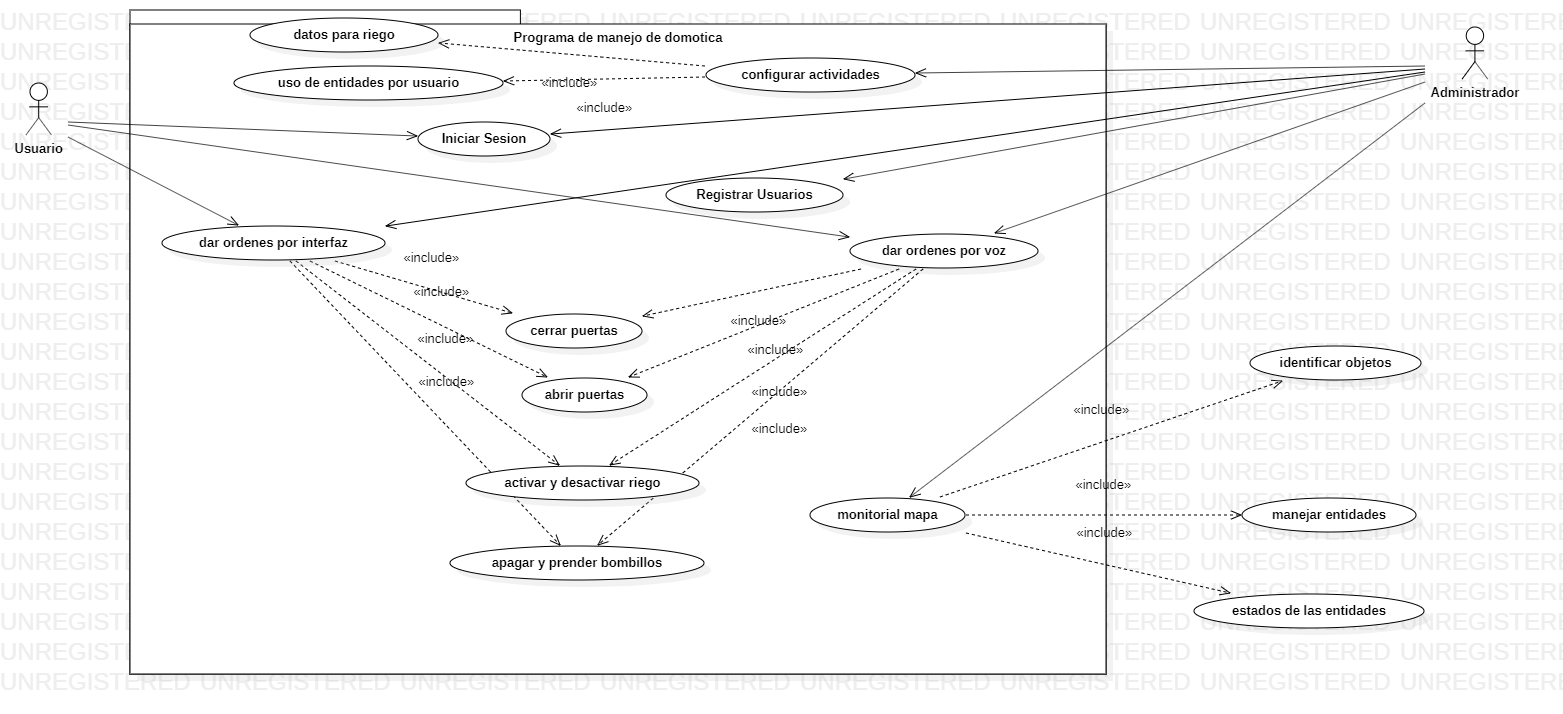
\includegraphics[width=\linewidth]{staruml/img/caso-de-uso-1.png}
  \caption{Casos de uso interfaz grafica}
  \label{fig:Casos de uso para manejo de cliente}
\end{figure}\\